%! suppress = NonBreakingSpace
%! BibTeX Compiler = biber

% Preamble
\documentclass[10pt]{article}
\title{LudS 24/25 Klausur I}
\author{Christoph Derszteler}

% Packages
\usepackage[T1]{fontenc}
\usepackage{lmodern}
\usepackage{bbding} % Required for '\Checkmark' symbol
\usepackage[ngerman]{babel}
\usepackage[
  a4paper,
  left=2cm,
  right=2cm,
  top=3cm,
  bottom=3cm
]{geometry}
\usepackage[small]{titlesec}
\usepackage[bottom]{footmisc}
\usepackage{float}
\usepackage{setspace}
\interfootnotelinepenalty=100000
\usepackage{blindtext}

\usepackage[hidelinks]{hyperref}
\hypersetup{
  linkcolor=black,
  linktoc=all,
}

\usepackage{graphicx}
\usepackage{booktabs}
\usepackage{gensymb}
\usepackage{siunitx}
\usepackage{amsfonts}
\usepackage{amsmath}
\usepackage{amssymb}
\usepackage{mathtools}
\usepackage{cancel}
\usepackage{stmaryrd} % Required for lightning symbol
\usepackage{xcolor}
\usepackage{tikz}
\usetikzlibrary{automata,positioning}
\sisetup{
  group-separator = {,},
  input-decimal-markers={,},
  output-decimal-marker = {,},
  exponent-product={\ensuremath{\cdot}}
}

\counterwithin*{equation}{section}
\counterwithin*{figure}{section}

\renewcommand{\thesection}{Aufgabe \arabic{section}: }

\renewcommand{\labelenumi}{(\alph{enumi})}
\renewcommand{\labelenumii}{(\arabic{enumii})}
\renewcommand{\labelenumiii}{(\roman{enumiii})}

\newcommand{\sectiontitle}{}
\newcommand{\newsection}[2]{\renewcommand{\sectiontitle}{#1}\section{#1}\label{sec:#2}}

\usepackage{fancyhdr}
\usepackage{pdfpages}
\pagestyle{fancy}
\lhead{Matrikelnummer: }
\rhead{}
\cfoot{\thepage}
\renewcommand{\headrulewidth}{0.4pt}

\usepackage{ifthen}
\usepackage{wasysym}
\newboolean{showsolutions}
\setboolean{showsolutions}{false}
\newcommand{\solution}[2]{
  \ifthenelse{\boolean{showsolutions}}
    {\color{olive} #1 \color{black}}  % Show solution if showsolutions is true
    {#2}  % Show blank space if showsolutions is false
}
\newcommand{\correctsquare}{\solution{\boxtimes}{\square}}

% Document
\begin{document}
  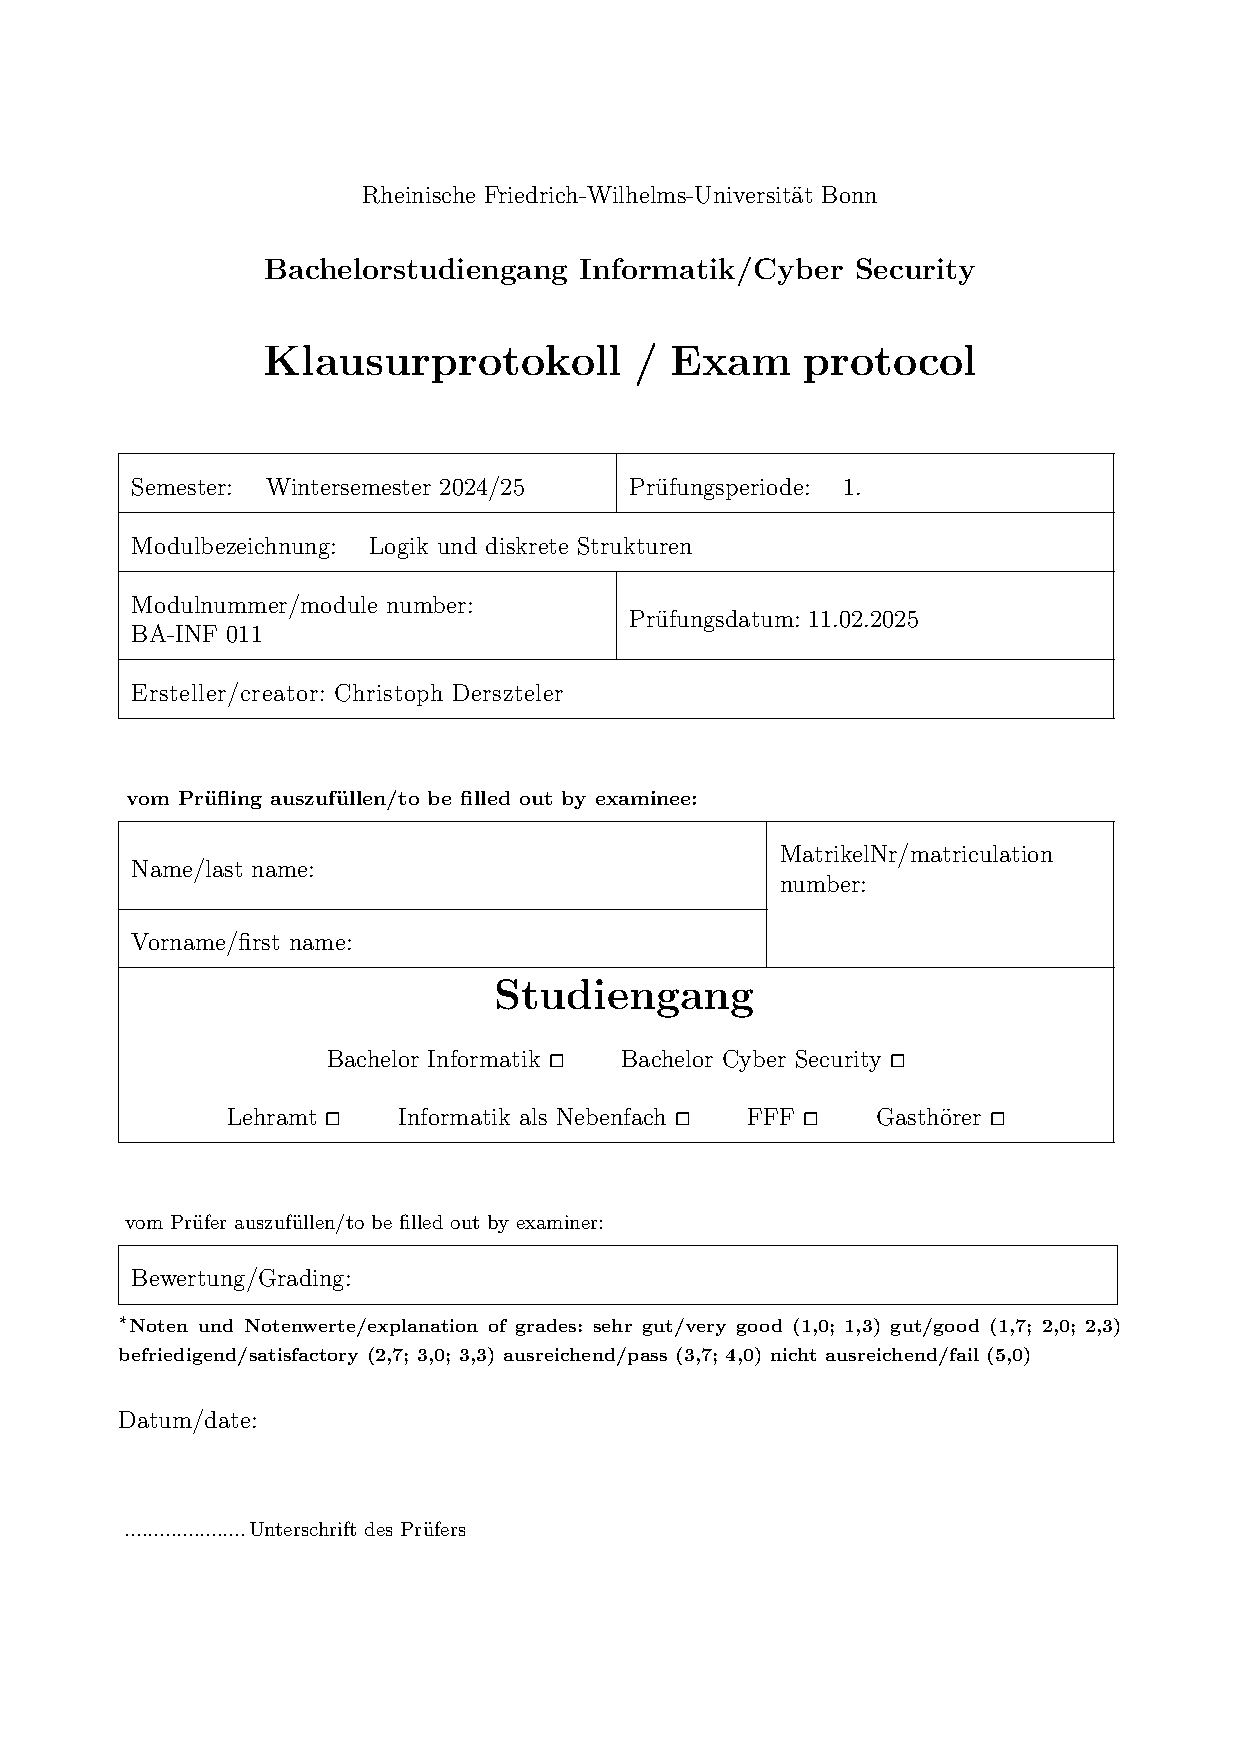
\includepdf[pages=-]{external/cover.pdf}
  
\includepdf[pages=-]{external/front-page.pdf}

  \newsection{Mengen, Relationen und Abbildungen}{task-1}

\begin{enumerate}
  \item {
    Es seien N, M zwei Mengen mit $|N| = n, |M| = m$ und $|N \setminus M| = d$.
    Geben Sie die folgenden Kardinalitäten an.
    Begründen Sie Ihre Antwort kurz, indem Sie die Zwischenschenschritte angeben.
    \begin{enumerate}
      \item $|\mathcal{P}(M \cup N)| = $ \vspace*{4cm}
      \item $|(M \cap N) \times M| = $ \vspace*{4cm}
    \end{enumerate}
  }
  \item {
    Zeigen Sie mittels vollständiger Induktion, dass für alle $n \in \mathbb{N}$
    gilt:
    \[
      \sum_{i=0}^{n-1} (3i^2 + 3i + 1) = n^3
    \]
  }
  \newpage
  \item {
    Kreuzen Sie für jede der folgenden Funktionen an, ob sie \textit{injektiv},
    \textit{surjektiv} oder \textit{weder noch} ist.
    Eine Begründung ist \textit{nicht} notwendig.

    \setlength{\tabcolsep}{10pt}
    \renewcommand{\arraystretch}{2}
    \begin{tabular}{@{}l c c c@{}}
      & $f$ injektiv & $f$ surjektiv & $f$ weder injektiv noch surjektiv \\
      $f: \mathbb{R} \to \mathbb{R} $ mit $f(x) = x^2 - 2x$ & $\square$ & $\square$ & $\square$ \\
      $f: \mathcal{P}(\mathbb{N}) \to \mathbb{N}_0 $ mit $f(A) = |A|$ & $\square$ & $\square$ & $\square$ \\[10pt]
      $f: \mathbb{R} \to \mathbb{R} $ mit $f(x) =
        \begin{cases}
          -(x^2), & x \leq 0 \\
          x^2 & x > 0
        \end{cases}
        $ & $\square$ & $\square$ & $\square$ \\[10pt]
      $f: \mathbb{R}^2 \to \mathbb{R}^2 $ mit $f(x, y) = (y-7, \frac{1}{4} x)$ & $\square$ & $\square$ & $\square$ \\
      $f: \mathbb{R}^2_{\geq 0} \to \mathbb{R}_{\geq 0} $ mit $f(x, y) = x^y$ & $\square$ & $\square$ & $\square$ \\
      $f: \mathbb{N}^2 \to \mathbb{N} $ mit $f(x, y) = x^2 + y^2$ & $\square$ & $\square$ & $\square$
    \end{tabular}
  }
  \vspace{\fill}
  \item {
    Seien $M = \{A, B, C, D\}$ eine Menge und $R \subseteq M \times M$ die unten
    schematisch dargestellte Relation auf $M$. Geben Sie jeweils mit
    \textit{kurzer} Begründung an, ob $R$ reflexiv, symmetrisch, transitiv,
    antisymmetrisch bzw. eine Äquivalenzrelation ist.

    \begin{center}
    \begin{tikzpicture}[node distance=2cm, auto]
      \node[state] (A)  {$A$};
      \node[state] (B) [right=of A]  {$B$};
      \node[state] (C) [below=of A]  {$C$};
      \node[state] (D) [below=of B]  {$D$};
      \path[->]
      (A) edge [bend left =15] node {} (B)
      (B) edge [bend right =-15] node {} (A)
      (A) edge [bend left =15] node {} (C)
      (C) edge [bend right =-15] node {} (A)
      (B) edge [bend left =15] node {} (D)
      (D) edge [bend right =-15] node {} (B)
      (B) edge [bend left =15] node {} (C)
      (C) edge [bend right =-15] node {} (B);
    \end{tikzpicture}
    \end{center}
    \vspace{\fill}

    \begin{minipage}{\linewidth}
      reflexiv: \hrulefill \\[10pt]
      symmetrisch: \hrulefill \\[10pt] \hrule \vspace{18pt}
      transitiv: \hrulefill \\[10pt] \hrule \par\vspace{18pt}
      antisymmetrisch: \hrulefill \\[10pt] \hrule \par\vspace{18pt}
      Äquivalenzrelation: \hrulefill
    \end{minipage}
  }
  \vspace{\fill}
\end{enumerate}
  \newsection{Reguläre Sprachen und Automaten}{task-2}

\newcommand{\statement}[1]{
  \item{
    \noindent\begin{minipage}[t]{0.65\linewidth} % Left side (text)
      #1
    \end{minipage}
    \hfill
    \begin{minipage}[t]{0.31\linewidth} % Right side
      \vfill % Used to center vertically
      \begin{center}
        \setlength{\tabcolsep}{10pt} % Sets the column padding
        \begin{tabular}{@{}c c@{}}
          Wahr & Falsch \\
          $\square$ & $\square$
        \end{tabular}
      \end{center}
      \vfill % Used to center vertically
    \end{minipage}

    \vspace{10pt}
    \begin{minipage}{\linewidth}
    Begründung: \hrulefill \\[10pt] \hrule \vspace{20pt} \hrule
    \end{minipage}
  }
}

\begin{enumerate}
  \item {
    Geben Sie für den folgenden regulären Ausdruck die \textbf{Ableitungsregeln}
    einer Grammatik an.
    Verwenden Sie dabei so \textbf{wenige Regeln} wie möglich.

    \[
      R = b(aa + b)^*
    \]

    \vspace{10pt}

    Ableitungsregeln:
  }
  \vspace{\fill}
  \item {
    Zeichnen Sie für die folgende Sprache einen Deterministischen Endlichen
    Automaten (DFA) als Zustandsübergangsdiagramm:

    \[
      L = \{w \in \{0, 1\}^*\mathbin{:} w \text{~beginnt mit 1 und endet auf 0}\}
    \]
  }
  \vspace{\fill}
  \newpage
  \item {
    Geben sind die vier folgenden Aussagen über reguläre Sprachen.
    Entscheiden Sie jeweils, ob diese Aussagen wahr oder falsch sind und geben
    Sie eine Begründung an.

    \begin{enumerate}
      \setlength\itemsep{10pt}
      \statement{
        Wenn es bei einem NFA mindestens einen Übergang gibt, sodass das gelesene
        $w \in \Sigma{^*}$ in einem verwerfenden Zustand landet,
        so akzeptiert der NFA $w$ nicht.
      }
      \statement{
        Ein minimaler NFA hat höchstens so viele Zustände wie ein DFA,
        der die gleiche Sprache entscheidet, mit minimaler Anzahl an Zuständen.
      }
      \statement{
        Sei $k \in \mathbb{N}$ beliebig, aber fest.
        Jede Sprache, die nur Wörter der Länge $k$ akzeptiert, ist regulär.
      }
      \statement{
        Jede nicht reguläre Sprache kann durch das Pumping-Lemma auch als solche
        identifiziert werden.
      }
    \end{enumerate}
  }
  \newpage
  \item {
    Beweisen Sie mit Hilfe des Pumping-Lemmas, dass folgende Sprache über dem
    Alphabet $\Sigma = \{a, b\}$ nicht regulär ist:

    \[
      L = \{w \in \Sigma ~| ~|w|_a = |w|_b + 1\}
    \]
  }
\end{enumerate}
  \newsection{Mathematische Konzepte}{task-3}

\begin{enumerate}
  \item {
    Sei $S = \{2, 5, 8, 11, 14\}$ eine Menge.
    Zeigen Sie mittels Diagonalisierung, dass die Menge \\
    $M = \{f~|~f: \mathbb{N} \to S\}$ nicht abzählbar unendlich ist, ohne die
    Überabzählbarkeit anderer Mengen zu nutzen.
  }
  \newpage
  \item {
    Bestimmen Sie mit Hilfe des chinesischen Restsatzes eine Zahl
    $x \in \mathbb{Z}$ mit $x \equiv 3$ mod $12$ und $x \equiv 4$ mod $7$.
    Geben Sie dazu ihre Zwischenschritte und das finale Ergebnis an.
  }
  \vfill
  \item {
    Wie viele verschiedene Worte kann man durch Permutation des Wortes WASSEREIS
    bilden?
    Begründen Sie ihre Rechnung kurz!
    Sie brauchen das Ergbnis nicht auszurechnen.
  }
  \vfill
  \newpage
  \item {
    Sei $G \coloneq \text{Abb}(\mathbb{R})$ die Menge aller Funktionen
    $f: \mathbb{N} \to \mathbb{N}$.
    Im Folgenden seien $f_1$ und $f_2$ zwei beliebige Funktionen aus $G$ und
    $n \in \mathbb{N}$ beliebig.
    Wir betrachten die folgende Verknüpfung auf diesre Menge:

    \[
      (G, \sim) \text{~mit~} (f_1 \sim f_2)(n) = f_1(n) \cdot f_2(n).
    \]

    Geben Sie für diese Struktur an, ob es sich um eine Halbgruppe, ein Monoid,
    eine Gruppe oder keines von alledem handelt und ob die Verknüpfung kommutativ
    ist.
    Begründen Sie Ihre Antworten.
  }
\end{enumerate}
  \newsection{Mathematische Logik und Beweisführung}{task-4}

\begin{enumerate}
  \item{
    Vera hat in diesem Wintersemester angefangen zu studieren und bereits ihre
    ersten Vorlesungen gehört.
    Sie mag dabei manche Vorlesungen lieber als andere.

    Folgende Aussagen über {\glqq}Vera mag Vorlesung ...{\grqq} sind bereits bekannt:

    {
      \renewcommand{\labelenumii}{(\roman{enumii})}
      \begin{enumerate}
        \item{Vera mag Vorlesung-1 nicht.}
        \item{Wenn Vera Vorlesung-2 nicht mag und Vorlesung-3 mag, dann mag sie auch Vorlesung-1.}
        \item{Vera mag Vorlesung-3 oder sie mag Vorlesung-2 nicht.}
      \end{enumerate}
    }

    Die Aussagen sollen als Aussagenlogische Formeln formuliert werden.

    \begin{enumerate}
      \item {
        Geben Sie geeignte Variablen und deren Bedeutung für die Aussagen an!

        \solution{
          V1: Vera mag Vorlesung-1 \\
          V2: Vera mag Vorlesung-2 \\
          V3: Vera mag Vorlesung-3
        }{\vfill}
      }
      \item {
        Formulieren Sie die Aussagen mit den Variablen als
        \textbf{syntaktisch korrekte Aussagenlogische Formeln}.
        \begin{enumerate}
          \item{
            \solution{
              $\varphi_1 = \neg V1$
            }{}
          }
          \item{
            \solution{
              $\varphi_2 = ((\neg V2 \wedge V3) \to V1)$
            }{\vspace{20pt}}
          }
          \item{
            \solution{
              $\varphi_3 = (\neg V2 \vee V3)$
            }{\vspace{20pt}}
          }
        \end{enumerate}
        \solution{}{\vspace{20pt}} % The spacing is weird, which is why we have to shift all vspaces by one item
      }
      \item {
        Finden Sie eine Bewertung, mit der alle Regeln erfüllt sind.

        \solution{
          Mit $B(V1) = 0$ und $B(V2) = B(V3) = 1$ sind alle Regeln erfüllt.
        }{\vfill}
      }
      \item {
        Ist es möglich, dass alle Regeln erfüllt sind und Vera Vorlesung-2 anders
        bewertet als Vorlesung-3?
        Begründen Sie Ihre Antwort kurz mittels der Methodik aus der Vorlesung!

        \solution{
          Nein, dies ist nicht möglich. Damit Regel (i) erfüllt ist, muss $B(V1) = 0$ sein.
          Damit dann (ii) erfüllt ist, muss die Implikatiosnannahme falsch sein.
          Dies ist der Fall, wenn mindestens entweder $B(V2) = 1$ oder $B(V3) = 0$.
          Damit allerdings gleichzeitig (iii) erfüllt ist, muss die Bewertung der
          Variable, die in (ii) dafür sorgt, dass die Implikationsannahme falsch ist,
          die Disjunktion in (iii) erfüllen, also muss $B(V2) = 0$ oder $B(V3) = 1$ sein.

          Die folgende Wahrheitstabelle zeigt den Zusammenhang anschaulich:

          \vspace{10pt}
          \setlength{\tabcolsep}{5pt}
          \begin{center}
            \begin{tabular}{c|c||c|c||c|c}
              $V2$ & $V3$ & $(\neg V2 \wedge V3)$ & $(\neg V2 \vee V3)$ & $\varphi_2$ & $\varphi_3$ \\ \hline\hline
              0 & 0 & 0 & 1 & 1 & 1 \\
              0 & 1 & 1 & 1 & 0 & 1 \\
              1 & 0 & 0 & 0 & 1 & 0 \\
              1 & 1 & 0 & 1 & 1 & 1
            \end{tabular}
          \end{center}

          Wie zu sehen ist, ermöglicht nur eine gleiche Bewertung von $V2$ und $V3$,
          dass sowohol $\varphi_2$ als auch $\varphi_3$ erfüllt sind.
        }{\vfill}
      }
    \end{enumerate}
  }
  \newpage
  \item{
    Nun betrachten wir den korrekten Umgang mit Wertetabellen zur Aussagenlogik!
    Folgende Aussagenlogische Formeln sind gegeben:

    \[
      \varphi_1 = (X \wedge (Y \vee Z)) \quad
      \varphi_2 = ((X \wedge Y) \vee (X \wedge Z)) \quad
      \varphi = (\varphi_1 \leftrightarrow \varphi_2)
    \]

    \vspace{10pt}
    \begin{enumerate}
      \item {
        Welche allgemeingültige Aussagen wird durch $(\varphi_1 \leftrightarrow \varphi_2)$
        ausgedrückt?

        \solution{
          Die Allgemeingültigkeit von $(\varphi_1 \leftrightarrow \varphi_2)$
          drückt das Distributivgesetz der Disjunktion aus.
        }{\vspace{40pt}}
      }
      \item {
        Werten Sie die folgende Wahrheitstabelle aus, indem Sie die leeren
        Spalten mit \textbf{syntaktisch korrekten} Hilfsaussagen füllen!

        \vspace{10pt}
        \setlength{\tabcolsep}{10pt}
        \renewcommand{\arraystretch}{1.5}
        \begin{center}
          \begin{tabular}{c|c|c||c|c|c||c|c|c}
            $X$ & $Y$ & $Z$ & $(Y \vee Z)$ & \solution{$(X \wedge Y)$}{\hspace{60pt}} & \solution{$(X \wedge Z)$}{\hspace{60pt}} & $\varphi_1$ & $\varphi_2$ & $\varphi$ \\ \hline\hline
            0 & 0 & 0 & \solution{0}{} & \solution{0}{} & \solution{0}{} &\solution{0}{}  & \solution{0}{} & \solution{1}{} \\ \hline
            0 & 0 & 1 & \solution{1}{} & \solution{0}{} & \solution{0}{} &\solution{0}{}  & \solution{0}{} & \solution{1}{} \\ \hline
            0 & 1 & 0 & \solution{1}{} & \solution{0}{} & \solution{0}{} &\solution{0}{}  & \solution{0}{} & \solution{1}{} \\ \hline
            0 & 1 & 1 & \solution{1}{} & \solution{0}{} & \solution{0}{} &\solution{0}{}  & \solution{0}{} & \solution{1}{} \\ \hline
            1 & 0 & 0 & \solution{0}{} & \solution{0}{} & \solution{0}{} &\solution{0}{}  & \solution{0}{} & \solution{1}{} \\ \hline
            1 & 0 & 1 & \solution{1}{} & \solution{0}{} & \solution{1}{} &\solution{1}{}  & \solution{1}{} & \solution{1}{} \\ \hline
            1 & 1 & 0 & \solution{1}{} & \solution{1}{} & \solution{0}{} &\solution{1}{}  & \solution{1}{} & \solution{1}{} \\ \hline
            1 & 1 & 1 & \solution{1}{} & \solution{1}{} & \solution{1}{} &\solution{1}{}  & \solution{1}{} & \solution{1}{} \\ \hline
          \end{tabular}
        \end{center}
        \vspace{20pt}
      }
      \item {
        Wie lässt sich anhand dieser Wertetabelle erkennen, dass $\varphi$
        eine Tautologie ist?
        Begründen Sie kurz.

        \solution{
          Es lässt sich anhand der Wertetabelle erkennen, dass $\varphi$ immer
          wahr (1) und somit unabhängig von den Bewertungen von $X, Y$ und $Z$
          ist.
          Das macht $\varphi$ definitionsgemäß zu einer Tautologie.
        }{}
      }
    \end{enumerate}
  }
  \newpage
  \item {
    Wir betrachten das Resolutionskalkül für Aussgnelogische Formeln und
    dessen Ableitungsregeln!

    Doktor Halbschlau hat sich für das Resolutionskalkül der Aussagenlogik
    folgende neue Ableitungsregeln ausgedacht.

    Aus zwei beliebige Klauseln $C_1, C_2$ entsteht immer und ohne Bedingungen
    in einem einzigen Resolutionsschritt eine neue Klausel
    \[
      C = C_1 \cup C_2
    \]

    Die Abbildung zeigt ein ganz einfaches Beispiel der Anwendung dieser Regel:

    \begin{center}
      \begin{tikzpicture}[distance = 2cm]
        \node (c1) {$C_1 = \{\neg X, Z\}$};
        \node (c) [right=of c1, below=1.5cm] {$C = \{\neg X, Z, Y, W\}$};
        \node (c2) [right=of c, above=1.5cm] {$C_2 = \{\neg X, Y, W\}$};

        \draw (c1) -- (c);
        \draw (c2) -- (c);
        % below=2cm
      \end{tikzpicture}
    \end{center}

    \vspace{20pt}
    Seien $C_1 = \{\neg x_1, x_2\},\: C_2 = \{x_1\}$ und $C_3 = \{\neg x_1, x_3\}$ Klauseln.

    \begin{enumerate}
      \item {
        Für eine Klauselmenge $K$ ist Res$^1(K)$ wie folgt definiert.
        Geben Sie konkret die neuen Resolventen an, die sich aus dem
        Resolutionskalkül von Doktor Halbschlau für $C_1, C_2$ und $C_3$
        ableiten lassen!

        \vspace{10pt}
        \[
          \solution{}{\hspace{-120pt}} \text{Res}^1(K) \coloneq \text{Res}(K)
            = K \cup \{ \solution{\{\neg x_1, x_1\}, \{\neg x_1, x_3\}, \{x_1, x_3\} \} }{}
        \]
        \vspace{10pt}
      }
      \item {
        Geben Sie nun auch die Definition von Res$^2(K)$ \textit{und}
        die konkreten Resolventen, die sich im 2. Schritt ableiten lassen, an.

        \vspace{10pt}
        \[
          \solution{}{\hspace{-60pt}} \text{Res}^2(K) \coloneq \solution{\text{Res}(\text{Res}^1(K))}{\hspace{120pt}} = \solution{\text{Res}^1(K) \cup \{\}}{\hspace{60pt} \cup \; \{}
        \]
        \vspace{10pt}
      }
      \item {
        Ab welchem $n \in \mathbb{N}$ gilt Res$^n(K) =$ Res$^*(K)$?
        Geben Sie jenes $n$ an und begründen Sie in einem \textbf{einzigen Satz}!

        \solution{
          Ab $n=1 \in \mathbb{N}$ gilt Res$^n(K) =$ Res$^*(K)$, da im 2. Schritt (s.o.)
          keine neuen Resolventen ableitbar waren, also Res$^1(K) =$ Res$^2(K)$.
        }{}
      }
    \end{enumerate}
  }
  \newpage
  \item {
    Wir wollen uns mit der Korrektheit und der Vollständigkeit des
    vorhin vorgestellten Resolutionskalküls von Doktor Halbschlau beschäftigen.

    \begin{enumerate}
      \item {
        Beweisen Sie allgemein anhand einer Bewertung $B$ und deren Bedeutung,
        dass, wenn die Klauseln $\{C_1, C_2\}$ erfüllt sind, auch immer die
        Klauselmenge $\{C_1, C_2, C\}$ erfüllt ist.

        \solution{
          Wenn die Klauselmenge $\{C_1, C_2\}$ erfüllt ist, müssen definitionsgemäß
          jeweils alle Klauseln, also $C_1$ und $C_2$ erfüllt sein.
          Dafür muss mindestens ein Literal aus je einer Klausel erfüllt sein.
          Damit dies der Fall ist, muss für eine Bewertung eines Literals $l \in C$
          $B(l) = 1$, sofern $l$ ein positives Literal ist, oder $B(l) = 0$,
          sofern $l$ ein negatives Literal ist, gelten.

          Die abgeleitete Klausel $C$ enthält nach der Ableitungsregel des
          Resolutionskalküls alle Literale aus $C_1$ und $C_2$.
          Da bereits die Klauselmenge $\{C_1, C_2\}$ erfüllt ist und somit jeweils
          mindestens ein Literal aus $C_1$ und $C_2$ erfüllt sind, ist auch
          mindestens ein Literal aus $C$ erfüllt.
          Somit ist $C$ und damit auch die Klauselmenge $\{C_1, C_2, C\}$ erfüllt.
        }{\vfill}
      }
      \item {
        Beweisen oder widerlegen Sie in einem \textbf{einzigen Satz}, dass
        die Ableitungsregeln des Resolutionskalküls \textit{korrekt} im Sinne der
        Vorlesung sind.

        \solution{
          Da, wie oben gezeigt, alle abgeleiteten Klauseln aus zwei erfüllten Klauseln
          ebenfalls erfüllt sind, werden nur wahre Aussagen abgeleitet und
          das Resolutionskalkül ist definitionsgemäß korrekt.
        }{\vspace{50pt}}
      }
      \item {
        Zeigen Sie anhand eines kleinen Beispiels, dass das Resolutionskalkül
        nicht \textit{vollständig} im Sinne der Vorlesung ist.

        \solution{
          Seien $C_1 = \{\neg x_1, x_2\}$ und $C_1 = \{x_1, x_2\}$ Klauseln.

          Mittels dem aus der Vorlesung bekannten Resolutionskalkül lässt sich
          die wahre Klausel $C = \{x_2\}$ ableiten.
          Aus dem Resolutionskalkül von Doktor Halbschlau lässt sich allerdings
          nur die Klausel $C' = \{\neg x_1, x_1, x_2\}$ ableiten.

          Somit lassen sich aus dem gegebenen Resolutionskalkül nicht alle
          wahren Aussagen ableiten und das Resolutionskalkül ist nicht vollständig
          im Sinne der Vorlesung.
        }{\vfill \vfill}
      }
    \end{enumerate}
  }
\end{enumerate}

  \setboolean{showsolutions}{true}

  \newsection{Mengen, Relationen und Abbildungen}{task-1}

\begin{enumerate}
  \item {
    Es seien N, M zwei Mengen mit $|N| = n, |M| = m$ und $|N \setminus M| = d$.
    Geben Sie die folgenden Kardinalitäten an.
    Begründen Sie Ihre Antwort kurz, indem Sie die Zwischenschenschritte angeben.
    \begin{enumerate}
      \item $|\mathcal{P}(M \cup N)| = $ \vspace*{4cm}
      \item $|(M \cap N) \times M| = $ \vspace*{4cm}
    \end{enumerate}
  }
  \item {
    Zeigen Sie mittels vollständiger Induktion, dass für alle $n \in \mathbb{N}$
    gilt:
    \[
      \sum_{i=0}^{n-1} (3i^2 + 3i + 1) = n^3
    \]
  }
  \newpage
  \item {
    Kreuzen Sie für jede der folgenden Funktionen an, ob sie \textit{injektiv},
    \textit{surjektiv} oder \textit{weder noch} ist.
    Eine Begründung ist \textit{nicht} notwendig.

    \setlength{\tabcolsep}{10pt}
    \renewcommand{\arraystretch}{2}
    \begin{tabular}{@{}l c c c@{}}
      & $f$ injektiv & $f$ surjektiv & $f$ weder injektiv noch surjektiv \\
      $f: \mathbb{R} \to \mathbb{R} $ mit $f(x) = x^2 - 2x$ & $\square$ & $\square$ & $\square$ \\
      $f: \mathcal{P}(\mathbb{N}) \to \mathbb{N}_0 $ mit $f(A) = |A|$ & $\square$ & $\square$ & $\square$ \\[10pt]
      $f: \mathbb{R} \to \mathbb{R} $ mit $f(x) =
        \begin{cases}
          -(x^2), & x \leq 0 \\
          x^2 & x > 0
        \end{cases}
        $ & $\square$ & $\square$ & $\square$ \\[10pt]
      $f: \mathbb{R}^2 \to \mathbb{R}^2 $ mit $f(x, y) = (y-7, \frac{1}{4} x)$ & $\square$ & $\square$ & $\square$ \\
      $f: \mathbb{R}^2_{\geq 0} \to \mathbb{R}_{\geq 0} $ mit $f(x, y) = x^y$ & $\square$ & $\square$ & $\square$ \\
      $f: \mathbb{N}^2 \to \mathbb{N} $ mit $f(x, y) = x^2 + y^2$ & $\square$ & $\square$ & $\square$
    \end{tabular}
  }
  \vspace{\fill}
  \item {
    Seien $M = \{A, B, C, D\}$ eine Menge und $R \subseteq M \times M$ die unten
    schematisch dargestellte Relation auf $M$. Geben Sie jeweils mit
    \textit{kurzer} Begründung an, ob $R$ reflexiv, symmetrisch, transitiv,
    antisymmetrisch bzw. eine Äquivalenzrelation ist.

    \begin{center}
    \begin{tikzpicture}[node distance=2cm, auto]
      \node[state] (A)  {$A$};
      \node[state] (B) [right=of A]  {$B$};
      \node[state] (C) [below=of A]  {$C$};
      \node[state] (D) [below=of B]  {$D$};
      \path[->]
      (A) edge [bend left =15] node {} (B)
      (B) edge [bend right =-15] node {} (A)
      (A) edge [bend left =15] node {} (C)
      (C) edge [bend right =-15] node {} (A)
      (B) edge [bend left =15] node {} (D)
      (D) edge [bend right =-15] node {} (B)
      (B) edge [bend left =15] node {} (C)
      (C) edge [bend right =-15] node {} (B);
    \end{tikzpicture}
    \end{center}
    \vspace{\fill}

    \begin{minipage}{\linewidth}
      reflexiv: \hrulefill \\[10pt]
      symmetrisch: \hrulefill \\[10pt] \hrule \vspace{18pt}
      transitiv: \hrulefill \\[10pt] \hrule \par\vspace{18pt}
      antisymmetrisch: \hrulefill \\[10pt] \hrule \par\vspace{18pt}
      Äquivalenzrelation: \hrulefill
    \end{minipage}
  }
  \vspace{\fill}
\end{enumerate}
  \newsection{Reguläre Sprachen und Automaten}{task-2}

\newcommand{\statement}[1]{
  \item{
    \noindent\begin{minipage}[t]{0.65\linewidth} % Left side (text)
      #1
    \end{minipage}
    \hfill
    \begin{minipage}[t]{0.31\linewidth} % Right side
      \vfill % Used to center vertically
      \begin{center}
        \setlength{\tabcolsep}{10pt} % Sets the column padding
        \begin{tabular}{@{}c c@{}}
          Wahr & Falsch \\
          $\square$ & $\square$
        \end{tabular}
      \end{center}
      \vfill % Used to center vertically
    \end{minipage}

    \vspace{10pt}
    \begin{minipage}{\linewidth}
    Begründung: \hrulefill \\[10pt] \hrule \vspace{20pt} \hrule
    \end{minipage}
  }
}

\begin{enumerate}
  \item {
    Geben Sie für den folgenden regulären Ausdruck die \textbf{Ableitungsregeln}
    einer Grammatik an.
    Verwenden Sie dabei so \textbf{wenige Regeln} wie möglich.

    \[
      R = b(aa + b)^*
    \]

    \vspace{10pt}

    Ableitungsregeln:
  }
  \vspace{\fill}
  \item {
    Zeichnen Sie für die folgende Sprache einen Deterministischen Endlichen
    Automaten (DFA) als Zustandsübergangsdiagramm:

    \[
      L = \{w \in \{0, 1\}^*\mathbin{:} w \text{~beginnt mit 1 und endet auf 0}\}
    \]
  }
  \vspace{\fill}
  \newpage
  \item {
    Geben sind die vier folgenden Aussagen über reguläre Sprachen.
    Entscheiden Sie jeweils, ob diese Aussagen wahr oder falsch sind und geben
    Sie eine Begründung an.

    \begin{enumerate}
      \setlength\itemsep{10pt}
      \statement{
        Wenn es bei einem NFA mindestens einen Übergang gibt, sodass das gelesene
        $w \in \Sigma{^*}$ in einem verwerfenden Zustand landet,
        so akzeptiert der NFA $w$ nicht.
      }
      \statement{
        Ein minimaler NFA hat höchstens so viele Zustände wie ein DFA,
        der die gleiche Sprache entscheidet, mit minimaler Anzahl an Zuständen.
      }
      \statement{
        Sei $k \in \mathbb{N}$ beliebig, aber fest.
        Jede Sprache, die nur Wörter der Länge $k$ akzeptiert, ist regulär.
      }
      \statement{
        Jede nicht reguläre Sprache kann durch das Pumping-Lemma auch als solche
        identifiziert werden.
      }
    \end{enumerate}
  }
  \newpage
  \item {
    Beweisen Sie mit Hilfe des Pumping-Lemmas, dass folgende Sprache über dem
    Alphabet $\Sigma = \{a, b\}$ nicht regulär ist:

    \[
      L = \{w \in \Sigma ~| ~|w|_a = |w|_b + 1\}
    \]
  }
\end{enumerate}
  \newsection{Mathematische Konzepte}{task-3}

\begin{enumerate}
  \item {
    Sei $S = \{2, 5, 8, 11, 14\}$ eine Menge.
    Zeigen Sie mittels Diagonalisierung, dass die Menge \\
    $M = \{f~|~f: \mathbb{N} \to S\}$ nicht abzählbar unendlich ist, ohne die
    Überabzählbarkeit anderer Mengen zu nutzen.
  }
  \newpage
  \item {
    Bestimmen Sie mit Hilfe des chinesischen Restsatzes eine Zahl
    $x \in \mathbb{Z}$ mit $x \equiv 3$ mod $12$ und $x \equiv 4$ mod $7$.
    Geben Sie dazu ihre Zwischenschritte und das finale Ergebnis an.
  }
  \vfill
  \item {
    Wie viele verschiedene Worte kann man durch Permutation des Wortes WASSEREIS
    bilden?
    Begründen Sie ihre Rechnung kurz!
    Sie brauchen das Ergbnis nicht auszurechnen.
  }
  \vfill
  \newpage
  \item {
    Sei $G \coloneq \text{Abb}(\mathbb{R})$ die Menge aller Funktionen
    $f: \mathbb{N} \to \mathbb{N}$.
    Im Folgenden seien $f_1$ und $f_2$ zwei beliebige Funktionen aus $G$ und
    $n \in \mathbb{N}$ beliebig.
    Wir betrachten die folgende Verknüpfung auf diesre Menge:

    \[
      (G, \sim) \text{~mit~} (f_1 \sim f_2)(n) = f_1(n) \cdot f_2(n).
    \]

    Geben Sie für diese Struktur an, ob es sich um eine Halbgruppe, ein Monoid,
    eine Gruppe oder keines von alledem handelt und ob die Verknüpfung kommutativ
    ist.
    Begründen Sie Ihre Antworten.
  }
\end{enumerate}
  \newsection{Mathematische Logik und Beweisführung}{task-4}

\begin{enumerate}
  \item{
    Vera hat in diesem Wintersemester angefangen zu studieren und bereits ihre
    ersten Vorlesungen gehört.
    Sie mag dabei manche Vorlesungen lieber als andere.

    Folgende Aussagen über {\glqq}Vera mag Vorlesung ...{\grqq} sind bereits bekannt:

    {
      \renewcommand{\labelenumii}{(\roman{enumii})}
      \begin{enumerate}
        \item{Vera mag Vorlesung-1 nicht.}
        \item{Wenn Vera Vorlesung-2 nicht mag und Vorlesung-3 mag, dann mag sie auch Vorlesung-1.}
        \item{Vera mag Vorlesung-3 oder sie mag Vorlesung-2 nicht.}
      \end{enumerate}
    }

    Die Aussagen sollen als Aussagenlogische Formeln formuliert werden.

    \begin{enumerate}
      \item {
        Geben Sie geeignte Variablen und deren Bedeutung für die Aussagen an!

        \solution{
          V1: Vera mag Vorlesung-1 \\
          V2: Vera mag Vorlesung-2 \\
          V3: Vera mag Vorlesung-3
        }{\vfill}
      }
      \item {
        Formulieren Sie die Aussagen mit den Variablen als
        \textbf{syntaktisch korrekte Aussagenlogische Formeln}.
        \begin{enumerate}
          \item{
            \solution{
              $\varphi_1 = \neg V1$
            }{}
          }
          \item{
            \solution{
              $\varphi_2 = ((\neg V2 \wedge V3) \to V1)$
            }{\vspace{20pt}}
          }
          \item{
            \solution{
              $\varphi_3 = (\neg V2 \vee V3)$
            }{\vspace{20pt}}
          }
        \end{enumerate}
        \solution{}{\vspace{20pt}} % The spacing is weird, which is why we have to shift all vspaces by one item
      }
      \item {
        Finden Sie eine Bewertung, mit der alle Regeln erfüllt sind.

        \solution{
          Mit $B(V1) = 0$ und $B(V2) = B(V3) = 1$ sind alle Regeln erfüllt.
        }{\vfill}
      }
      \item {
        Ist es möglich, dass alle Regeln erfüllt sind und Vera Vorlesung-2 anders
        bewertet als Vorlesung-3?
        Begründen Sie Ihre Antwort kurz mittels der Methodik aus der Vorlesung!

        \solution{
          Nein, dies ist nicht möglich. Damit Regel (i) erfüllt ist, muss $B(V1) = 0$ sein.
          Damit dann (ii) erfüllt ist, muss die Implikatiosnannahme falsch sein.
          Dies ist der Fall, wenn mindestens entweder $B(V2) = 1$ oder $B(V3) = 0$.
          Damit allerdings gleichzeitig (iii) erfüllt ist, muss die Bewertung der
          Variable, die in (ii) dafür sorgt, dass die Implikationsannahme falsch ist,
          die Disjunktion in (iii) erfüllen, also muss $B(V2) = 0$ oder $B(V3) = 1$ sein.

          Die folgende Wahrheitstabelle zeigt den Zusammenhang anschaulich:

          \vspace{10pt}
          \setlength{\tabcolsep}{5pt}
          \begin{center}
            \begin{tabular}{c|c||c|c||c|c}
              $V2$ & $V3$ & $(\neg V2 \wedge V3)$ & $(\neg V2 \vee V3)$ & $\varphi_2$ & $\varphi_3$ \\ \hline\hline
              0 & 0 & 0 & 1 & 1 & 1 \\
              0 & 1 & 1 & 1 & 0 & 1 \\
              1 & 0 & 0 & 0 & 1 & 0 \\
              1 & 1 & 0 & 1 & 1 & 1
            \end{tabular}
          \end{center}

          Wie zu sehen ist, ermöglicht nur eine gleiche Bewertung von $V2$ und $V3$,
          dass sowohol $\varphi_2$ als auch $\varphi_3$ erfüllt sind.
        }{\vfill}
      }
    \end{enumerate}
  }
  \newpage
  \item{
    Nun betrachten wir den korrekten Umgang mit Wertetabellen zur Aussagenlogik!
    Folgende Aussagenlogische Formeln sind gegeben:

    \[
      \varphi_1 = (X \wedge (Y \vee Z)) \quad
      \varphi_2 = ((X \wedge Y) \vee (X \wedge Z)) \quad
      \varphi = (\varphi_1 \leftrightarrow \varphi_2)
    \]

    \vspace{10pt}
    \begin{enumerate}
      \item {
        Welche allgemeingültige Aussagen wird durch $(\varphi_1 \leftrightarrow \varphi_2)$
        ausgedrückt?

        \solution{
          Die Allgemeingültigkeit von $(\varphi_1 \leftrightarrow \varphi_2)$
          drückt das Distributivgesetz der Disjunktion aus.
        }{\vspace{40pt}}
      }
      \item {
        Werten Sie die folgende Wahrheitstabelle aus, indem Sie die leeren
        Spalten mit \textbf{syntaktisch korrekten} Hilfsaussagen füllen!

        \vspace{10pt}
        \setlength{\tabcolsep}{10pt}
        \renewcommand{\arraystretch}{1.5}
        \begin{center}
          \begin{tabular}{c|c|c||c|c|c||c|c|c}
            $X$ & $Y$ & $Z$ & $(Y \vee Z)$ & \solution{$(X \wedge Y)$}{\hspace{60pt}} & \solution{$(X \wedge Z)$}{\hspace{60pt}} & $\varphi_1$ & $\varphi_2$ & $\varphi$ \\ \hline\hline
            0 & 0 & 0 & \solution{0}{} & \solution{0}{} & \solution{0}{} &\solution{0}{}  & \solution{0}{} & \solution{1}{} \\ \hline
            0 & 0 & 1 & \solution{1}{} & \solution{0}{} & \solution{0}{} &\solution{0}{}  & \solution{0}{} & \solution{1}{} \\ \hline
            0 & 1 & 0 & \solution{1}{} & \solution{0}{} & \solution{0}{} &\solution{0}{}  & \solution{0}{} & \solution{1}{} \\ \hline
            0 & 1 & 1 & \solution{1}{} & \solution{0}{} & \solution{0}{} &\solution{0}{}  & \solution{0}{} & \solution{1}{} \\ \hline
            1 & 0 & 0 & \solution{0}{} & \solution{0}{} & \solution{0}{} &\solution{0}{}  & \solution{0}{} & \solution{1}{} \\ \hline
            1 & 0 & 1 & \solution{1}{} & \solution{0}{} & \solution{1}{} &\solution{1}{}  & \solution{1}{} & \solution{1}{} \\ \hline
            1 & 1 & 0 & \solution{1}{} & \solution{1}{} & \solution{0}{} &\solution{1}{}  & \solution{1}{} & \solution{1}{} \\ \hline
            1 & 1 & 1 & \solution{1}{} & \solution{1}{} & \solution{1}{} &\solution{1}{}  & \solution{1}{} & \solution{1}{} \\ \hline
          \end{tabular}
        \end{center}
        \vspace{20pt}
      }
      \item {
        Wie lässt sich anhand dieser Wertetabelle erkennen, dass $\varphi$
        eine Tautologie ist?
        Begründen Sie kurz.

        \solution{
          Es lässt sich anhand der Wertetabelle erkennen, dass $\varphi$ immer
          wahr (1) und somit unabhängig von den Bewertungen von $X, Y$ und $Z$
          ist.
          Das macht $\varphi$ definitionsgemäß zu einer Tautologie.
        }{}
      }
    \end{enumerate}
  }
  \newpage
  \item {
    Wir betrachten das Resolutionskalkül für Aussgnelogische Formeln und
    dessen Ableitungsregeln!

    Doktor Halbschlau hat sich für das Resolutionskalkül der Aussagenlogik
    folgende neue Ableitungsregeln ausgedacht.

    Aus zwei beliebige Klauseln $C_1, C_2$ entsteht immer und ohne Bedingungen
    in einem einzigen Resolutionsschritt eine neue Klausel
    \[
      C = C_1 \cup C_2
    \]

    Die Abbildung zeigt ein ganz einfaches Beispiel der Anwendung dieser Regel:

    \begin{center}
      \begin{tikzpicture}[distance = 2cm]
        \node (c1) {$C_1 = \{\neg X, Z\}$};
        \node (c) [right=of c1, below=1.5cm] {$C = \{\neg X, Z, Y, W\}$};
        \node (c2) [right=of c, above=1.5cm] {$C_2 = \{\neg X, Y, W\}$};

        \draw (c1) -- (c);
        \draw (c2) -- (c);
        % below=2cm
      \end{tikzpicture}
    \end{center}

    \vspace{20pt}
    Seien $C_1 = \{\neg x_1, x_2\},\: C_2 = \{x_1\}$ und $C_3 = \{\neg x_1, x_3\}$ Klauseln.

    \begin{enumerate}
      \item {
        Für eine Klauselmenge $K$ ist Res$^1(K)$ wie folgt definiert.
        Geben Sie konkret die neuen Resolventen an, die sich aus dem
        Resolutionskalkül von Doktor Halbschlau für $C_1, C_2$ und $C_3$
        ableiten lassen!

        \vspace{10pt}
        \[
          \solution{}{\hspace{-120pt}} \text{Res}^1(K) \coloneq \text{Res}(K)
            = K \cup \{ \solution{\{\neg x_1, x_1\}, \{\neg x_1, x_3\}, \{x_1, x_3\} \} }{}
        \]
        \vspace{10pt}
      }
      \item {
        Geben Sie nun auch die Definition von Res$^2(K)$ \textit{und}
        die konkreten Resolventen, die sich im 2. Schritt ableiten lassen, an.

        \vspace{10pt}
        \[
          \solution{}{\hspace{-60pt}} \text{Res}^2(K) \coloneq \solution{\text{Res}(\text{Res}^1(K))}{\hspace{120pt}} = \solution{\text{Res}^1(K) \cup \{\}}{\hspace{60pt} \cup \; \{}
        \]
        \vspace{10pt}
      }
      \item {
        Ab welchem $n \in \mathbb{N}$ gilt Res$^n(K) =$ Res$^*(K)$?
        Geben Sie jenes $n$ an und begründen Sie in einem \textbf{einzigen Satz}!

        \solution{
          Ab $n=1 \in \mathbb{N}$ gilt Res$^n(K) =$ Res$^*(K)$, da im 2. Schritt (s.o.)
          keine neuen Resolventen ableitbar waren, also Res$^1(K) =$ Res$^2(K)$.
        }{}
      }
    \end{enumerate}
  }
  \newpage
  \item {
    Wir wollen uns mit der Korrektheit und der Vollständigkeit des
    vorhin vorgestellten Resolutionskalküls von Doktor Halbschlau beschäftigen.

    \begin{enumerate}
      \item {
        Beweisen Sie allgemein anhand einer Bewertung $B$ und deren Bedeutung,
        dass, wenn die Klauseln $\{C_1, C_2\}$ erfüllt sind, auch immer die
        Klauselmenge $\{C_1, C_2, C\}$ erfüllt ist.

        \solution{
          Wenn die Klauselmenge $\{C_1, C_2\}$ erfüllt ist, müssen definitionsgemäß
          jeweils alle Klauseln, also $C_1$ und $C_2$ erfüllt sein.
          Dafür muss mindestens ein Literal aus je einer Klausel erfüllt sein.
          Damit dies der Fall ist, muss für eine Bewertung eines Literals $l \in C$
          $B(l) = 1$, sofern $l$ ein positives Literal ist, oder $B(l) = 0$,
          sofern $l$ ein negatives Literal ist, gelten.

          Die abgeleitete Klausel $C$ enthält nach der Ableitungsregel des
          Resolutionskalküls alle Literale aus $C_1$ und $C_2$.
          Da bereits die Klauselmenge $\{C_1, C_2\}$ erfüllt ist und somit jeweils
          mindestens ein Literal aus $C_1$ und $C_2$ erfüllt sind, ist auch
          mindestens ein Literal aus $C$ erfüllt.
          Somit ist $C$ und damit auch die Klauselmenge $\{C_1, C_2, C\}$ erfüllt.
        }{\vfill}
      }
      \item {
        Beweisen oder widerlegen Sie in einem \textbf{einzigen Satz}, dass
        die Ableitungsregeln des Resolutionskalküls \textit{korrekt} im Sinne der
        Vorlesung sind.

        \solution{
          Da, wie oben gezeigt, alle abgeleiteten Klauseln aus zwei erfüllten Klauseln
          ebenfalls erfüllt sind, werden nur wahre Aussagen abgeleitet und
          das Resolutionskalkül ist definitionsgemäß korrekt.
        }{\vspace{50pt}}
      }
      \item {
        Zeigen Sie anhand eines kleinen Beispiels, dass das Resolutionskalkül
        nicht \textit{vollständig} im Sinne der Vorlesung ist.

        \solution{
          Seien $C_1 = \{\neg x_1, x_2\}$ und $C_1 = \{x_1, x_2\}$ Klauseln.

          Mittels dem aus der Vorlesung bekannten Resolutionskalkül lässt sich
          die wahre Klausel $C = \{x_2\}$ ableiten.
          Aus dem Resolutionskalkül von Doktor Halbschlau lässt sich allerdings
          nur die Klausel $C' = \{\neg x_1, x_1, x_2\}$ ableiten.

          Somit lassen sich aus dem gegebenen Resolutionskalkül nicht alle
          wahren Aussagen ableiten und das Resolutionskalkül ist nicht vollständig
          im Sinne der Vorlesung.
        }{\vfill \vfill}
      }
    \end{enumerate}
  }
\end{enumerate}
\end{document}